% This literature review addresses the problem of real-time speaker counting in mono, overlapped, real-world audio. The aim is to identify existing solutions, highlight limitations, and position the proposed work within current research.

% Overlapping speech presents a major challenge in speech processing tasks such as diarisation and transcription. Accurate speaker counting is critical in environments with variable overlap densities, from no overlap to full concurrency.

% Speaker counting approaches vary between offline and real-time methods. Models have included convolutional neural networks, recurrent networks, convolutional-recurrent hybrids, and transformer-based architectures. Most focus on offline processing. It's important to stance that most methods are complex and a simple&lightweight method is missing from the research space.

% Many existing systems rely on multi-channel or far-field microphone setups. Mono input, while limited, is more realistic in consumer and embedded settings. The constraint forces models to learn from time-frequency patterns without spatial cues. (dont mention the models we've made in the lit review, this is just for context)

% Available datasets include LibriCSS, LibriMix, AMI, and others. These offer varying degrees of realism, overlap control, and microphone configuration. They do not target mono, real-time inference with realistic acoustic conditions. (LibriCSS is a re-recorded and modified version of the LibriSpeech dataset, generated by playing LibriSpeech audio through loudspeakers in a room and recording the playback using a seven-channel microphone array. This process introduces authentic spatial distortions into the data. (figures here))

% Prior work has focused on speaker counting using complex pipelines or multi-mic setups. Some explore CNNs on spectrograms for speaker activity detection. Others propose recurrent or CRN-based methods. Few operate on mono, single-segment audio in a truly real-time context.

% There is a clear gap in models designed for mono input with low-latency inference on real-world audio containing dynamic overlap. No current approach targets all of these constraints simultaneously.

% Applications include live meeting transcription, input to diarisation systems, or deployment on constrained hardware. These scenarios benefit from compact, accurate, and low-latency models.

% This work proposes a lightweight, mono-input model capable of real-time inference across varied overlap densities, addressing a critical gap in current literature.


% The below fig needs plugging somewhere when explaining what a spectrogram is.
% \begin{figure}[H]
%   \centering
%   \includegraphics[width=0.8\textwidth]{thesis/figs/Methodology/bat.png}
%   \caption{A spectrogram of a bat's echolocation \cite{bat_echolocation_jones}. Spectrograms are (recorded on the log-mel scale ... they are also temporal.... brighter areas are higher amplitude or volume...)}
%   \label{fig:bat_spec}
% \end{figure}


% what needs including:

% - what is speech processing - initial study by JP HATON \cite{earlySpeech1}
% - the typical speech processing pipeline and examples (create a figure and leave the png for me to add in \cite{pyannote2020} \cite{sp})
% - current successes and failures in speech processing
% - speaker counting and VAD as an upstream job in the pipeline; what are they? Why are they needed?
% - speaker counting and VAD progress in the field
% - issues with current models in real-time
% - a cnn approach will solve the production level issues
% - what is a cnn? (Insert a figure of an example CNN e.g. resnet50 \cite{ResNet50})
% - cnns will learn from spectrograms: what is a spectrogram?
% - ...
% -

% --------------------------------------------------------------------------------

\chapter{Literature Review}

Speech processing is the field concerned with the analysis and modelling of human vocal communication signals (\textbg{CITE}). Early studies by Haton and colleagues established speech processing as a formal research domain, focusing on speech recognition and the automatic extraction of linguistic information from acoustic input (\textbf{CITE}). Since then, the area has grown to encompass a wide range of tasks, including automatic speech recognition (ASR), speech enhancement, speaker diarisation, voice activity detection (VAD), and speaker counting.

A typical speech processing pipeline consists of several interconnected components designed to transform raw audio into structured information. These include front-end preprocessing (e.g., feature extraction from the waveform), segmentation (such as VAD), speaker analysis (e.g., diarisation or counting), and downstream tasks such as ASR (\textbf{CITE}).  illustrates the general structure of such a pipeline.

\begin{figure}[H]
\centering
\centerline{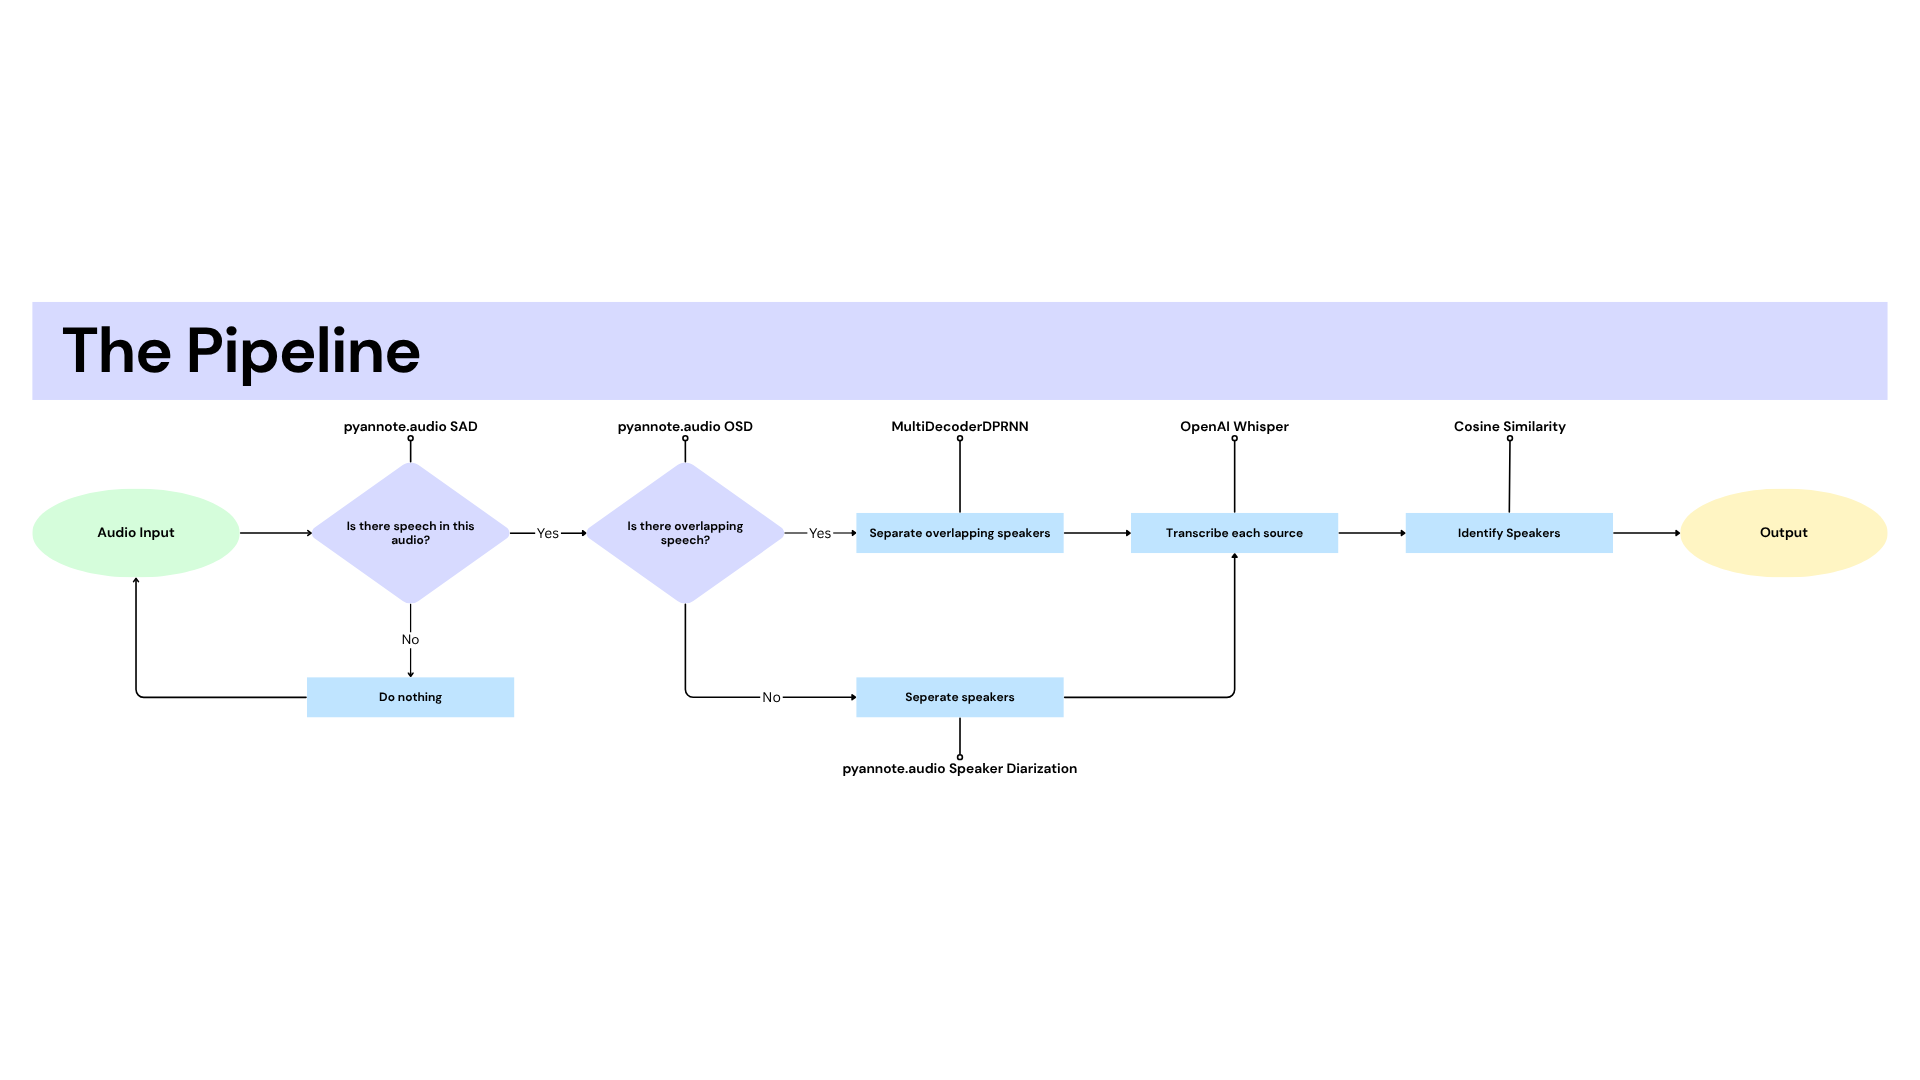
\includegraphics[scale=0.4]{figs/Intro&Review/FlowChart.png}}
\caption{A typical speech processing pipeline, making use of SOTA models \& methods \cite{pyannote2020, multidecoder_dprnn,openAIwhisper,cosine_similarity}. The end-goal of speech processing is to fully seperate and transcribe overlapping audio in a busy environment; each piece of the pipeline attempts a solution of one piece of the problem by assuming that previous parts are solved.}
\label{fig:pipeline}
\end{figure}

Advances in deep learning have led to impressive improvements in ASR and speaker diarisation, with transformer-based models achieving state-of-the-art results on large-scale datasets (\textbf{CITE}). However, successes in controlled or offline settings often do not generalise well to noisy, real-world, or resource-constrained environments (\textbf{CITE}).


VAD and speaker counting are key upstream components in the speech processing pipeline. VAD identifies whether speech is present in an audio segment, providing a foundation for segmentation and reducing computational load for subsequent modules (\textbf{CITE}). Speaker counting estimates the number of distinct concurrent speakers, which is especially important in overlapped speech scenarios where diarisation and ASR performance degrade significantly without accurate overlap detection (\textbf{CITE}).

Progress in VAD has been strong, with convolutional and recurrent architectures achieving near-human performance in controlled conditions (\textbf{CITE}). Speaker counting, however, remains more challenging due to the combinatorial complexity of overlapping voices. Existing methods include convolutional neural networks (CNNs) applied to spectrograms (\textbf{CITE}), recurrent neural networks for temporal modelling (\textbf{CITE}), convolutional-recurrent hybrids (\textbf{CITE}), and more recent transformer-based methods (\textbf{CITE}). Despite these advances, most approaches operate offline and assume access to multi-channel or far-field microphone arrays, limiting their applicability in consumer or embedded contexts (\textbf{CITE}).

Real-time processing introduces additional constraints: latency, robustness to dynamic overlap, and computational efficiency. Current systems often struggle to meet these requirements simultaneously. Many models rely on heavy architectures unsuited for deployment on embedded hardware, or require spatial information from multiple microphones that is unavailable in mono-channel scenarios (\textbf{CITE}). This creates a gap between academic research and production-level deployment.


CNNs provide a promising approach for lightweight, real-time speech processing. Originally popularised in computer vision tasks such as image classification and object detection (\textbf{CITE}), CNNs are well-suited for learning from spectrograms, which represent speech in a two-dimensional time-frequency space. A spectrogram encodes frequency content across time, with brighter regions representing higher amplitudes (see Figure~\ref{fig:bat_spec}). These features resemble images, making them naturally compatible with convolutional feature extractors.


\begin{figure}[H]
\centering
\includegraphics[width=0.8\textwidth]{figs/Intro&Review/resnet50.png}
\caption{a) An example of a state-of-the-art (SOTA) convolutional neural network (CNN) architecture \cite{ResNet50}. CNNs learn local patterns via convolutional filters and hierarchical feature maps. b) The types of residual block and the resulting feature map from each.}
\label{fig:cnn_example}
\end{figure}


\begin{figure}[H]
\centering
\includegraphics[width=0.8\textwidth]{figs/Intro&Review/bat.png}
\caption{A spectrogram of a bat's echolocation \cite{bat_echolocation_jones}. Spectrograms encode temporal and frequency information simultaneously, making them well-suited for CNN-based feature extraction.}
\label{fig:bat_spec}
\end{figure}


The suitability of CNNs for spectrogram analysis has led to their adoption in both VAD and speaker counting tasks. Unlike recurrent architectures, CNNs can achieve low-latency inference with fewer parameters, making them better suited for real-time deployment (\textbf{CITE}).


Several datasets support research in speaker overlap and counting, including LibriCSS, LibriMix, and the AMI corpus (\textbf{CITE}). LibriCSS is derived from LibriSpeech, replayed and re-recorded using microphone arrays to simulate realistic room acoustics (\textbf{CITE}). LibriMix provides mixtures of clean speech recordings with controlled overlap levels (\textbf{CITE}). However, these datasets are designed for multi-channel or offline processing and rarely target mono, low-latency inference in realistic acoustic environments.


While speaker counting has received attention in recent years, existing work is largely focused on offline, high-complexity methods, often assuming access to multi-microphone arrays. Real-time, mono-input processing in dynamic, overlapping conditions remains underexplored. This gap is critical for applications such as live transcription, meeting diarisation, and deployment on consumer hardware, where compact, low-latency, and robust models are essential.


\subsubsection{Summary}
CNN-based approaches offer a promising direction for lightweight, spectrogram-based feature extraction. However, there is a lack of models addressing the combined constraints of mono input, real-time inference, and robustness to dynamic overlap. The present work seeks to address this gap by developing and evaluating a compact CNN architecture optimised for real-time speaker counting in realistic, overlapped speech scenarios.